% \documentclass[12pt,journal,compsoc]{IEEEtran}
\documentclass[10pt,journal,compsoc]{IEEEtran}
\usepackage{graphicx}

\ifCLASSOPTIONcompsoc
\else
\fi

\ifCLASSINFOpdf
\else
\fi

\newcommand\MYhyperrefoptions{
bookmarks=true,bookmarksnumbered=true,
pdfpagemode={UseOutlines},plainpages=false,pdfpagelabels=true,
colorlinks=true,linkcolor={black},citecolor={black},urlcolor={black},
pdftitle={Rancang Bangun Robot Vision Untuk Object Finding Menggunakan Color Tracking pada perangkat RaspberryPi},
pdfsubject={Typesetting},
pdfauthor={Achmadi},
pdfkeywords={Kata Kunci}
}

\begin{document}


 \title{Rancang Bangun Robot Vision Untuk Object Finding Menggunakan Color Tracking pada perangkat RaspberryPi}

 \author{
 Achmadi, Apriani Kusuma Wardani\\
 Teknik Fisika, Fakultas Teknologi Industri, Institut Teknologi Sepuluh Nopember (ITS)\\
 Jl. Arief Rahman Hakim, Surabaya 60111\\
 \textit{Email:} mekatronik.achmadi@gmail.com, apriani.tf@gmail.com
%   Achmadi,241000085
%  \thanks{Dicetak 10 Desember 2014}
 }
 
%  \markboth{Handout Progres 1 TA Gasal 2014}{RapberryPi RoboVision}
 
%   \IEEEtitleabstractindextext{
%   
%   \begin{abstract}
%   Ini Abstrak.
%   \end{abstract}
%   
%   \begin{IEEEkeywords}
%   Ini Kata Kunci
%   \end{IEEEkeywords}
%   }
  
  \maketitle
%   \IEEEdisplaynontitleabstractindextext
%   \IEEEpeerreviewmaketitle
  
 
 \textbf{
 Abstrak--
 Telah dilakukan perancangan, pembangunan, dan pengujian sebuah robot berbasis vision yang mampu menemukan objek. 
 Robot dapat menemukan objek dengan target adalah bola berwarna biru dengan pengaturan rentang Hue adalah 100-130, Saturation 87-183, dan Value 80-182. 
 Dalam rentang ini robot dapat menemukan objek maximal pada jarak maximal 665 cm dan FOV 58 derajat dengan kecepatan roda antara 126-445 rpm. 
 Tingkat pencahayaan akan mempengaruhi nilai saturasi. Untuk warna lain membedakannya cukup dengan nilai Hue yaitu untuk merah pada 0-10, kuning pada 15-35, dan hijau pada 60-90.
 }
 
 \textbf{
 Kata Kunci--
 Robot Vision,
 RaspberrPi,
 HSV,
 Color Tracking
 }
 
 \begin{center}
     I. PENDAHULUAN
  \end{center}
  
  \IEEEPARstart{R}{obot} vision adalah robot yang mampu menggunakan kamera sebagai sumber informasi untuk diolah sesuai kebutuhan. 
  Tujuan utama setiap perancangan robot tentu adalah untuk mengganti pekerjaan manusia. 
  Kemampuan robot untuk melakukan pekerjaan yang berulang dan berbahaya telah menjadi kebutuhan di setiap lingkungan industri.
  Untuk memenuhi kebutuhan tersebut telah dikembangkan beragam teknologi sensor dan actuator. 
  Khusus untuk sensor, telah dikembangkan teknologi yang mirip dengan cara kerja pada indra manusia. 
  Salah satu yang banyak dipakai adalah penggunaan kamera sebagai pengganti mata untuk robot.
  Penggunaan kamera sebagai sensor visual telah banyak di terapkan pada bidang robotika.
  RaspberryPi merupakan salah satu jenis SBC (Single Board Computer) dengan spesifikasi processor BCM235 arsitektur arm1176 kategori armhf dan RAM 512. 
  Tersedia Operating System yang dapat dijalankan oleh RaspberryPi yaitu Raspbian yang berbasis Linux dan memiliki pustaka pengolahan citra OpenCV di lumbung perangkat lunaknya. 
  RaspberryPi dan Operating System Raspbian merupakan proyek opensource yang bersifat gratis.
  Pustaka OpenCV (Open Computer Vision) merupakan pustaka pemrograman berbasis C/C++/Python yang berisi fungsi-fungsi untuk akuisisi dan pengolahan citra.
  Penjejakan warna merupakan salah satu bentuk pengenalan objek yang cukup sederhana. 
  Prinsip proses penjejakan warna adalah mensegmentasi gambar sesuai warna kemudian membaca perubahan distribusi pixel hasil segmentasi.
  Mode warna HSV adalah mode warna yang menyatakan warna dalam 3 variabel yaitu Hue, Saturation, dan Value.
  Nilai Hue merepresentasikan nilai jenis warna yang merupakan nilai kombinasi RGB dalam besaran sudut. 
  Pada dasarnya nilai Hue dibagi dalam juring lingkaran sehingga jangkauan nilainya adalah 0-360, 
  namun karena dalam bahasa pemrograman variabel pemrograman hanya 8bit (0-255) maka jangkauan juring di reduksi menjadi setengah lingkaran (0-179).
  Segmentasi citra adalah proses mengumpulkan pixel-pixel karena kesamaan properti. 
  Kesamaan properti dapat berupa nilai intensitas, bentuk tekstur,garis tepi, dll. 
  Ada banyak teknik untuk segmentasi citra dengan masing-masing memiliki kompleksitas, kemampuan, dan penggunaannya.
  Proses segmentasi merupakan proses yang penting dalam pengolahan citra.
  Segmentasi digunakan untuk memfilter objek yang tidak dibutuhkan. 
  Filter dapat berupa persamaan matematis,logic maupun maupun matrix kernel.
  
  \begin{center}
     II. METODE PENELITIAN
  \end{center}
  
  \noindent \textit{A. Alur Penelitian}
  
  Pengerjaan tugas akhir ini meliputi studi literatur, perancangan dan pembangunan robot vision, pengujian robot vision, analisa data dan penyusunan laporan. 
  Tahapan pengerjaan tugas akhir ini dimulai dengan studi literatur. 
  Studi literatur ini bertujuan untuk mengetahui dasar-dasar perancangan robot yang telah dibuat pengembang lain.
  Disini desain robot yang dipilih adalah desain robot beroda karena desain terebut adalah desain yang paling mudah dan paling dasar. 
  Desain tersebut kemudian akan digunakan ketika perancangan. 
  Setelah desain selesai dibuat, maka robot akan dirakit menjadi 1 unit. 
  Setelah selesain perakitan, maka dilakukan proses penentuan nilai HSV sehingga robot dapat menemukan robot. 
  Jika ada kegagalan dalam pencarian objek, maka dilakukan perbaikan. 
  Kemudian unit tersebut akan di uji untuk mendapatkan spesifikasi dari robot itu sendiri mencakup jarak terjauh, jarak kiri-kanan,kecepatan, dan tingkat pencahayaan. 
  Setelah didapatkan data tersebut, maka akan dilakukan analisa. 
  Terakhir dilakukan penulisan laporan.
  Tahapan tersebut tergambar dalam diagram alir pada gambar 2.1 berikut:
  \begin{center}
    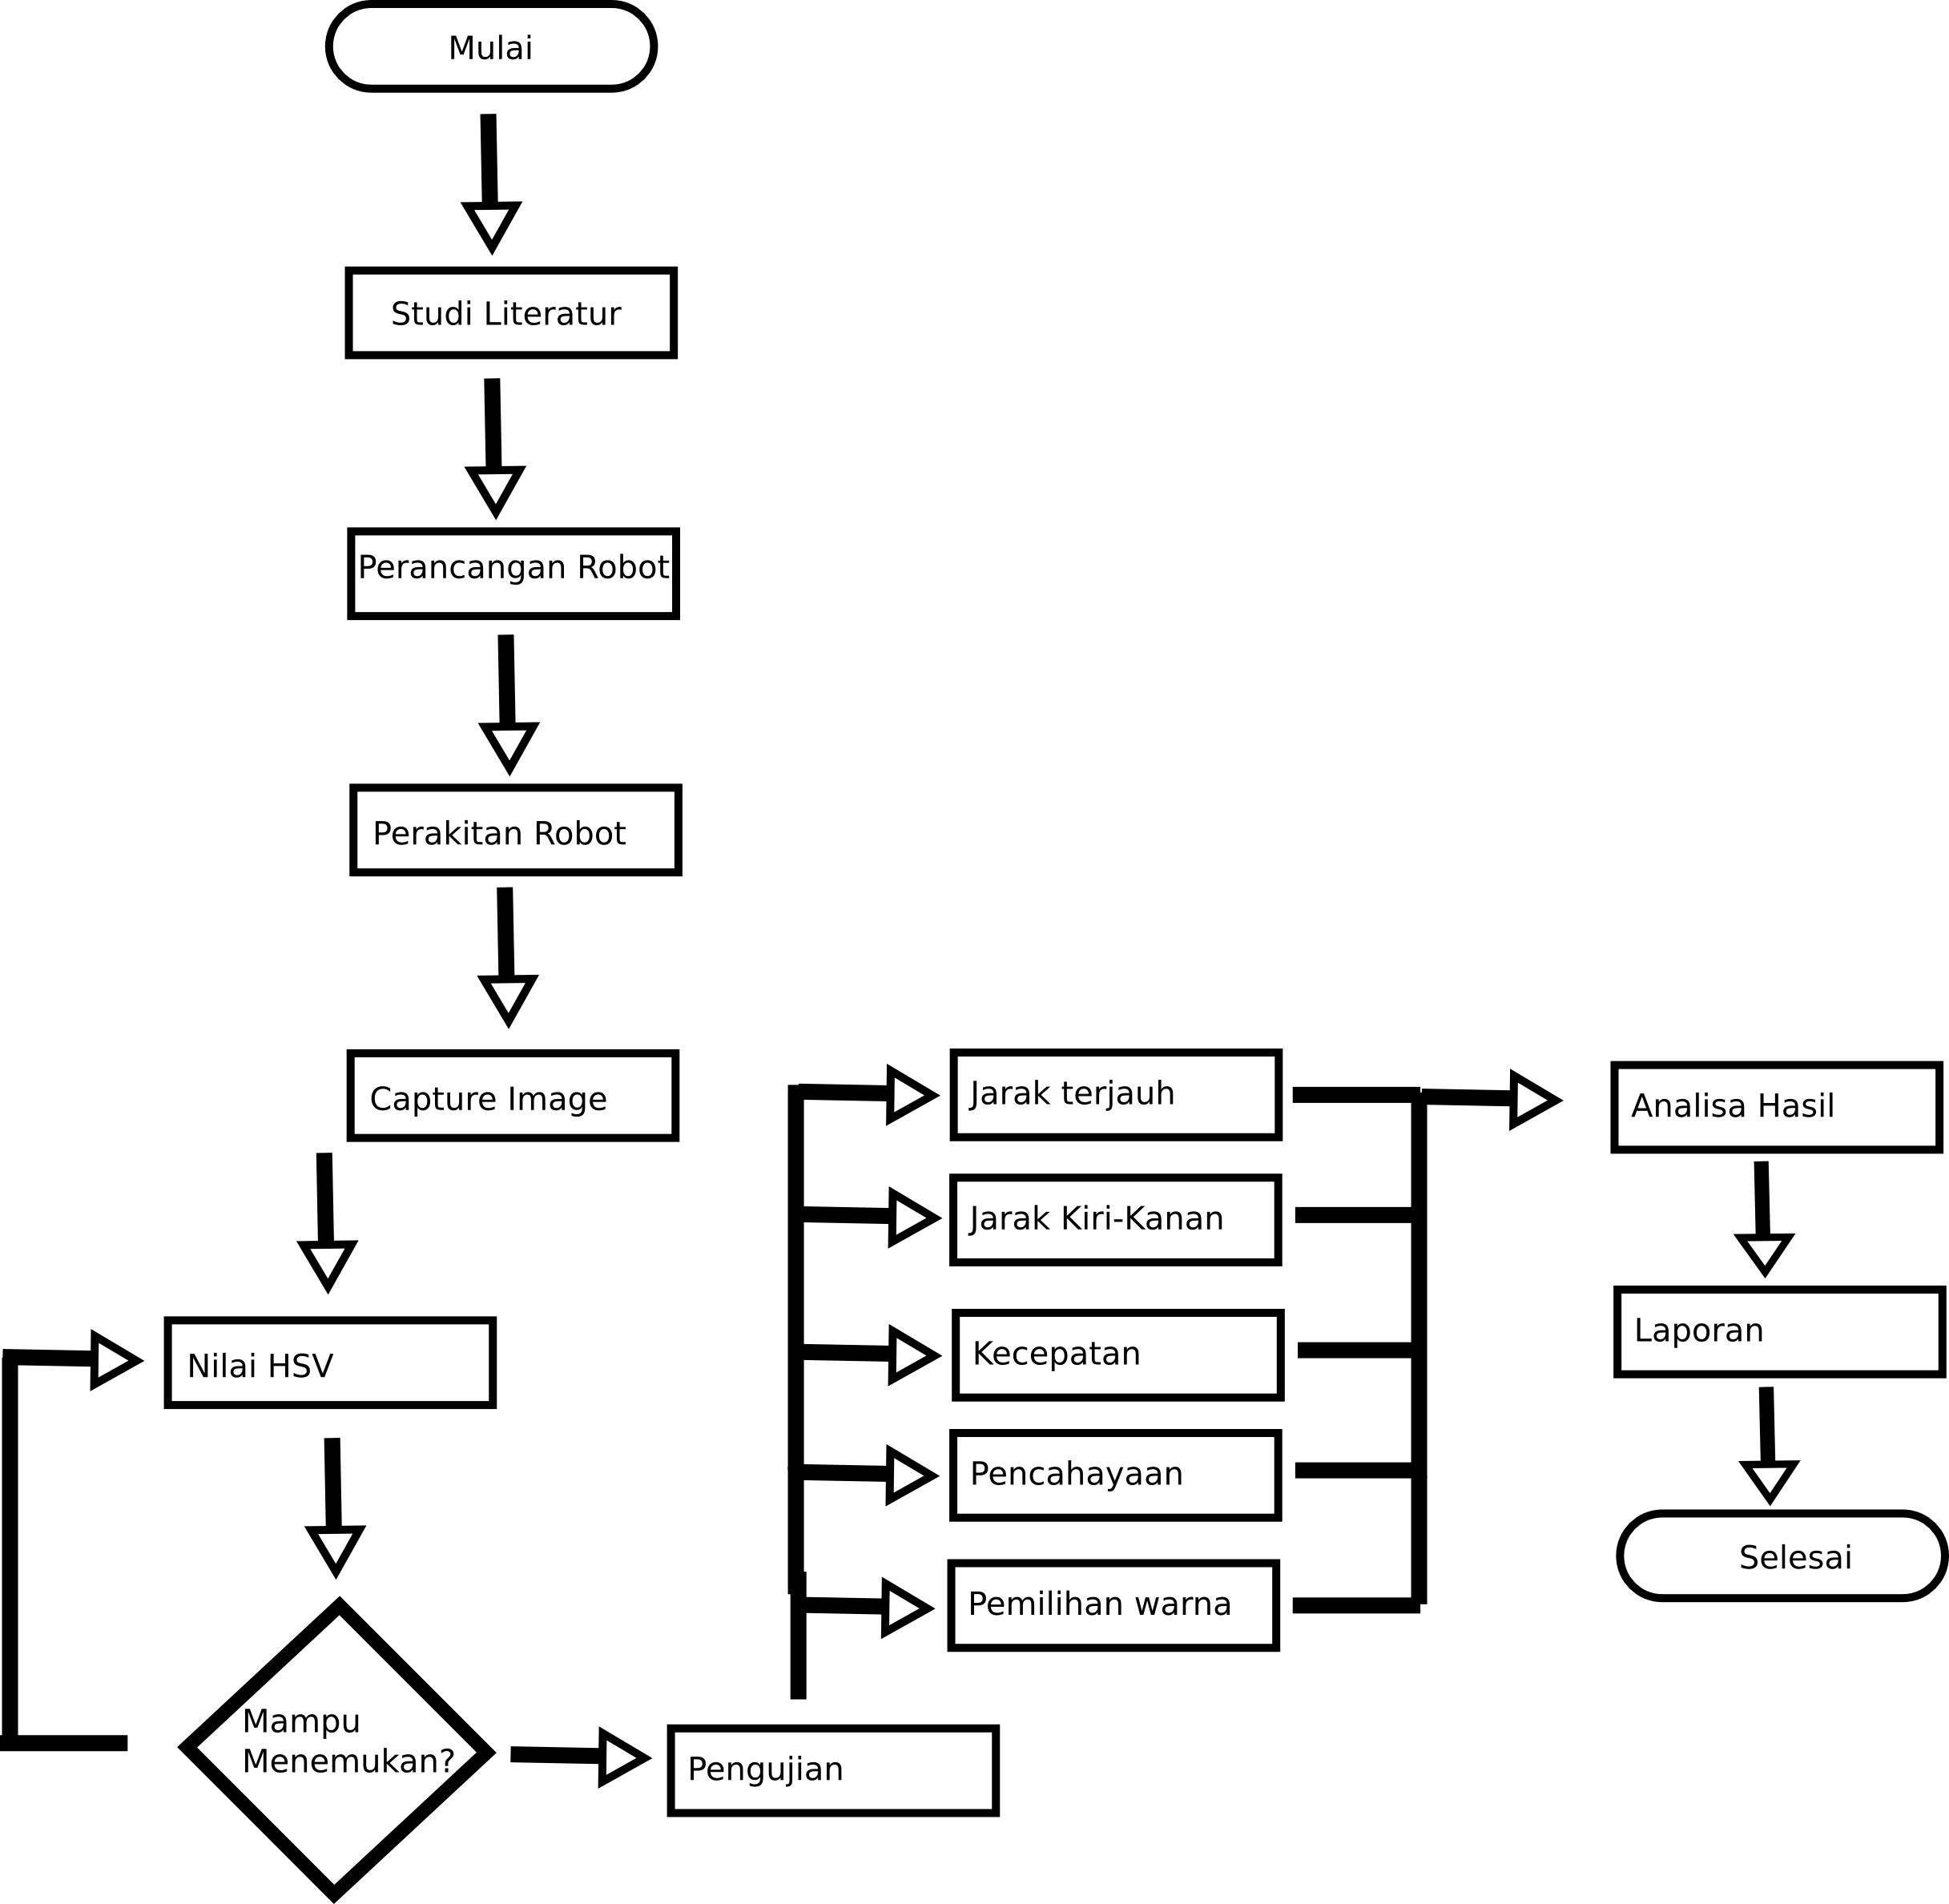
\includegraphics[width=250pt,height=350pt]{work}\\
    Gambar 1.1 Diagram alir kerja.
  \end{center}
  
  \noindent \textit{B. Perancangan dan Pembangunan}
  
  Perancangan robot dimulai dari mendesain sistem robot yang terbagi menjadi bagian yaitu:\\
  - Aktuator\\
  - Driver motor\\
  - Controller motor\\
  - Sistem tenaga\\
  - Algoritma perangkat lunak\\
  - Sedangkan untuk perangkat kamera dan RaspberryPi tidak perlu lagi dilakukan perancangan apa pun karena akan digunakan secara tanpa ada modifikasi.\\
  
  Setelah setiap bagian dibuat dan dirakit maka robot akan memiliki tampilan seperti pada gambar 2.2 berikut.
  
  \begin{center}
    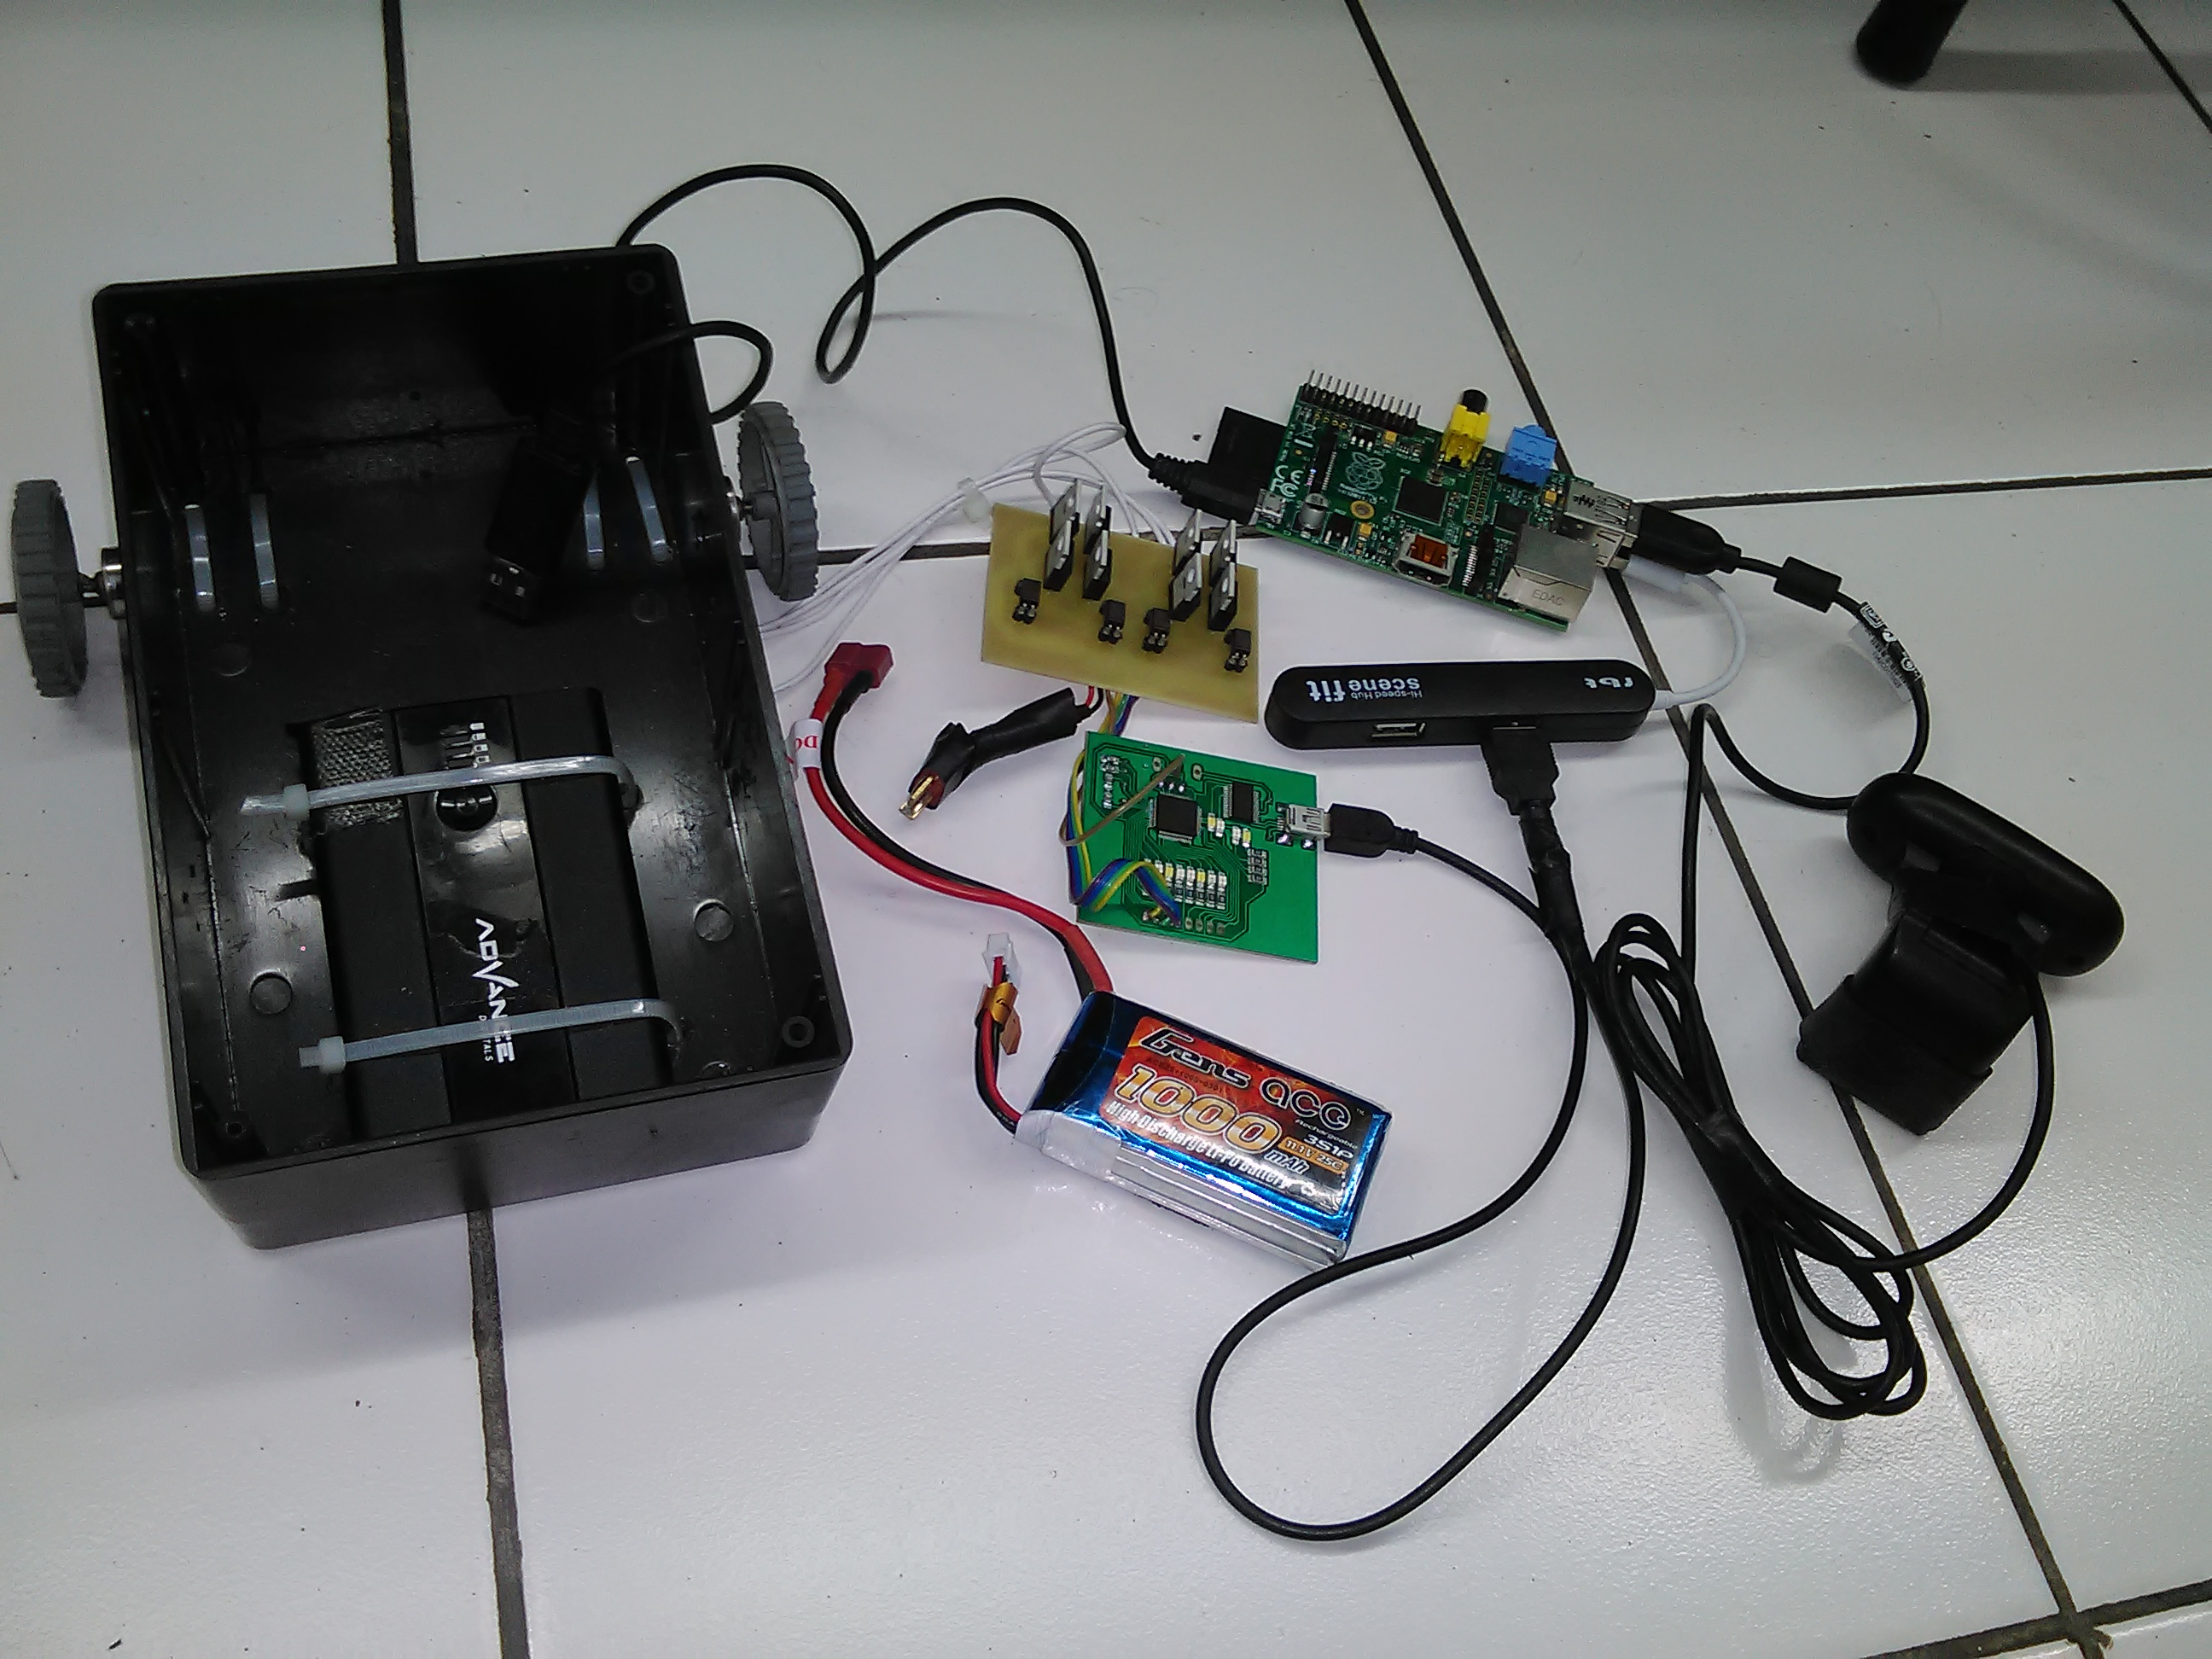
\includegraphics[width=200pt]{apart}\\
    Gambar 1.2 Bagian robot dalam keadaan belum menjadi satu
  \end{center}
  
  Sedangkan gambar 2.3 berikut adalah bagian robot yang dirakit menjadi satu.
  \begin{center}
    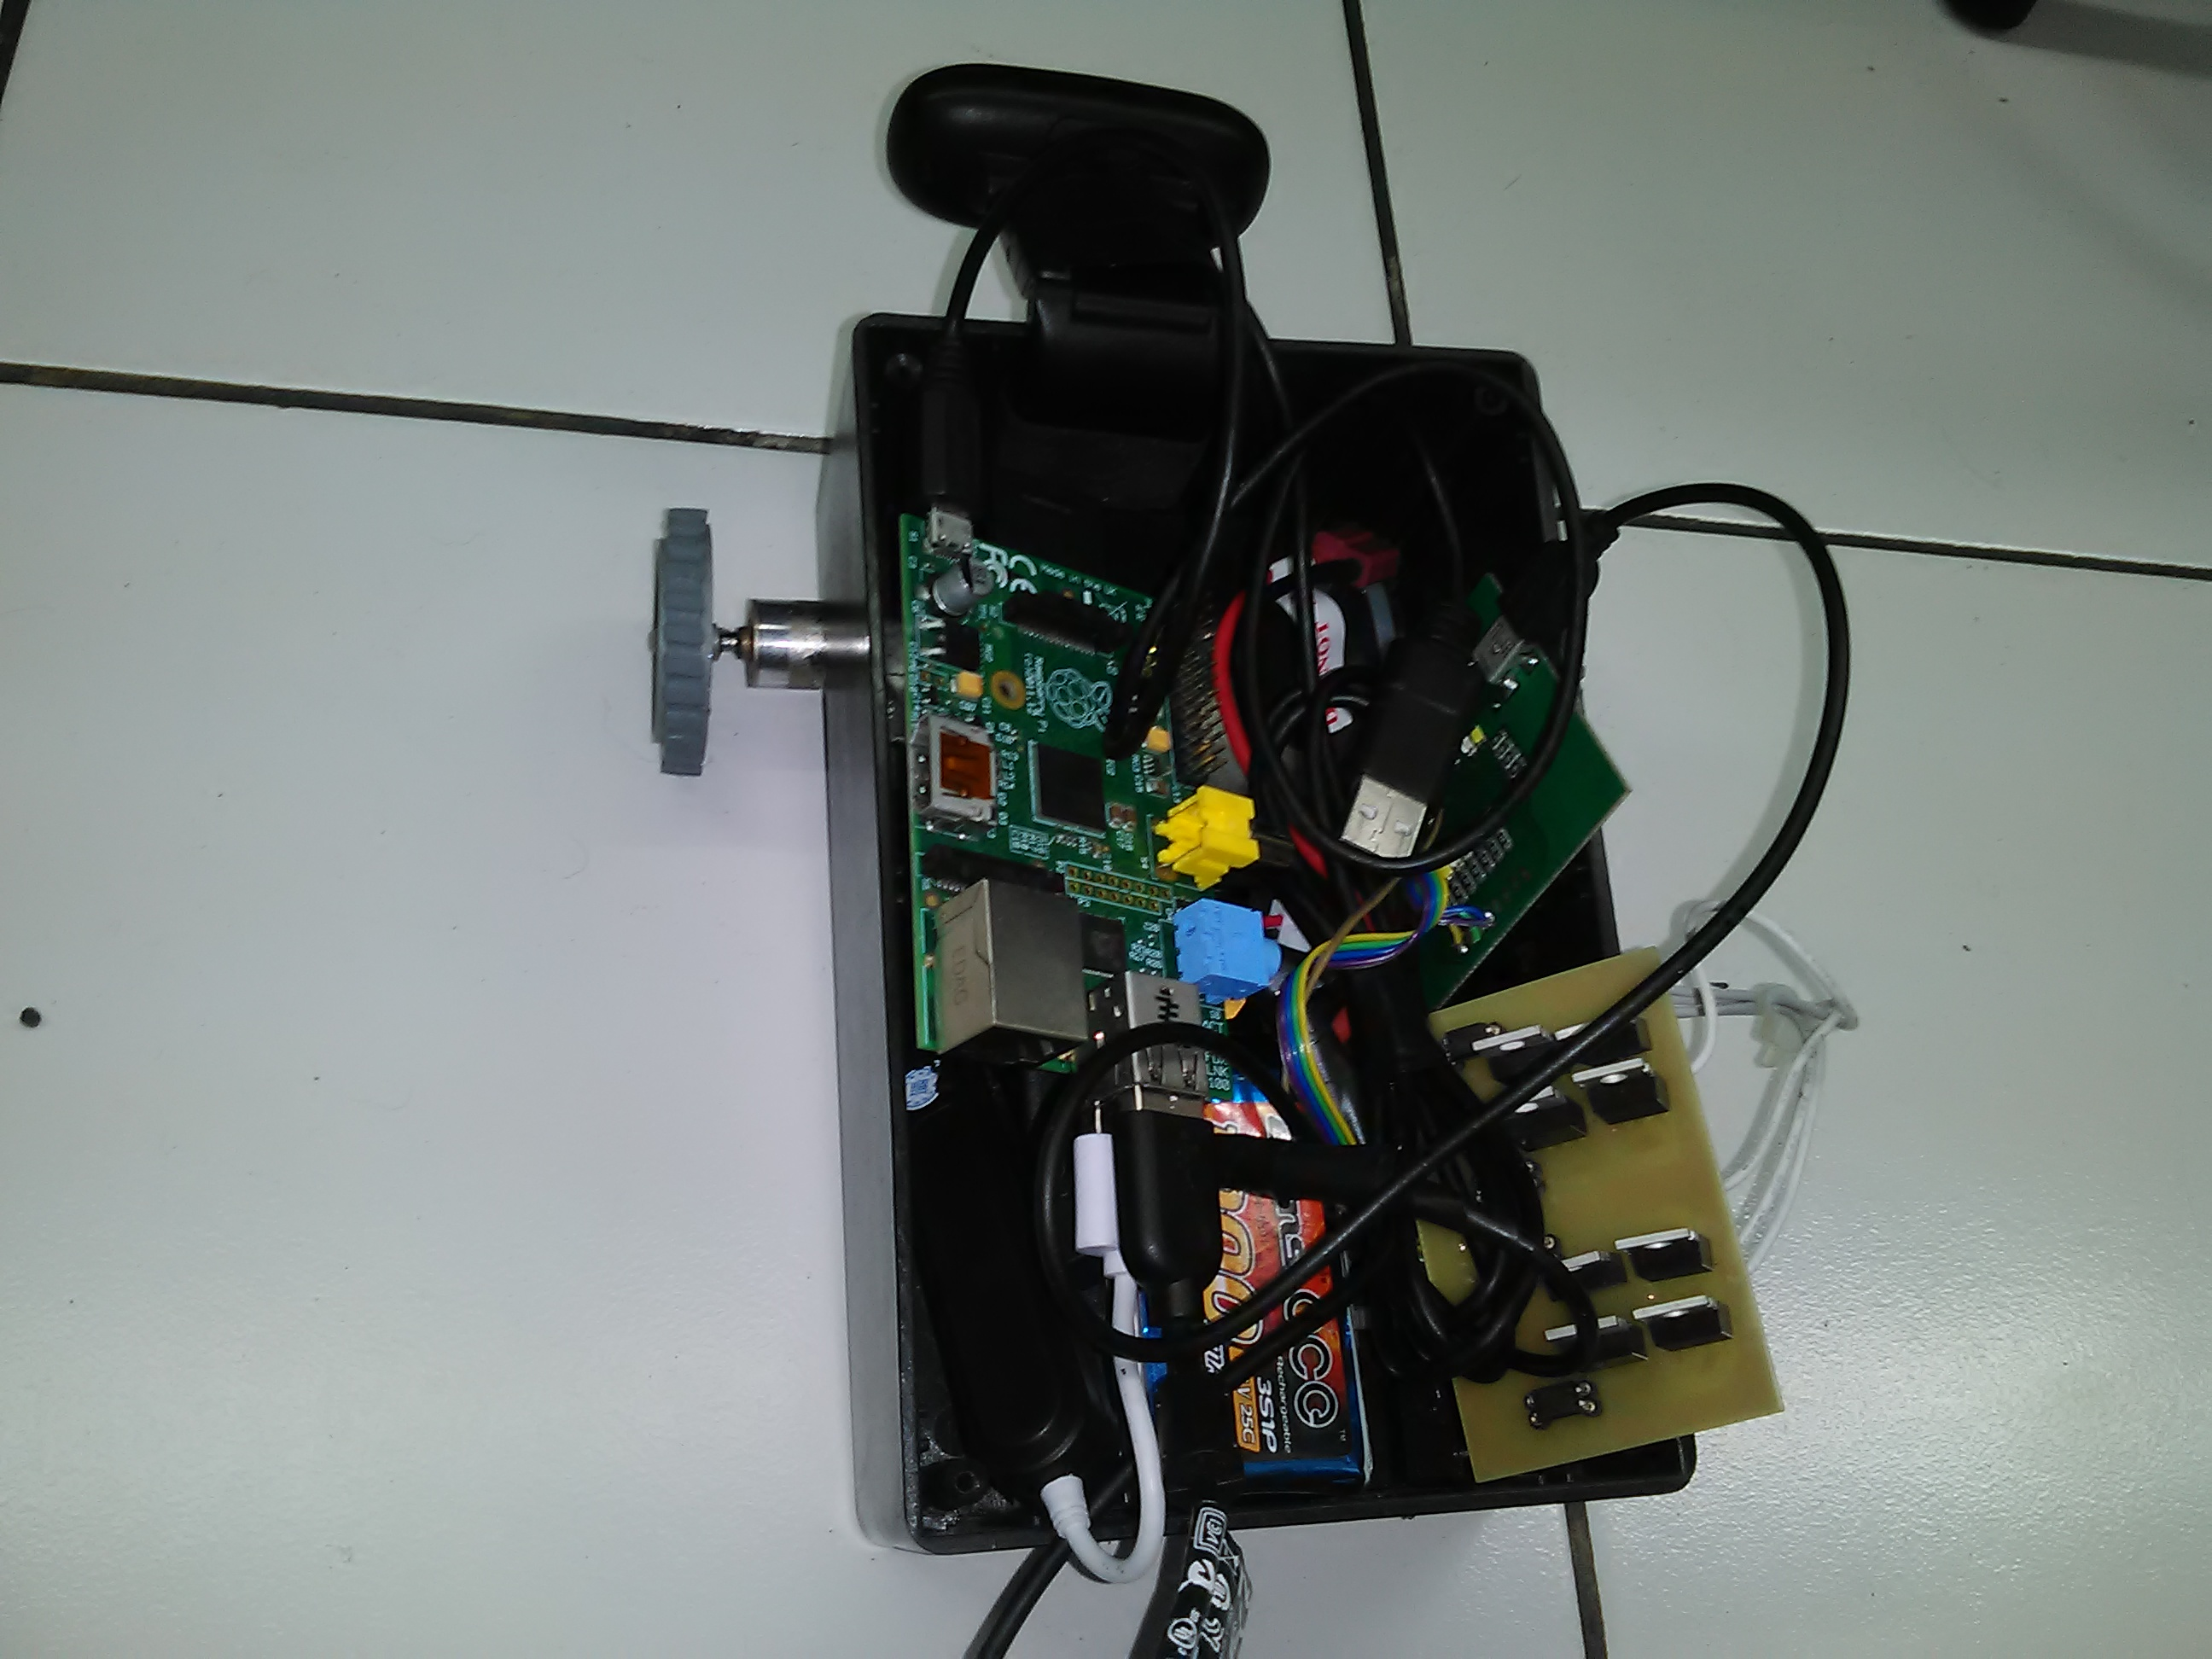
\includegraphics[width=200pt]{full}\\
    Gambar 1.3 Bagian robot dalam keadaan telah dirakit menjadi satu.
  \end{center}
  
  Untuk rancangan algoritma perangkat lunak ditunjukkan oleh gambar 2.4 berikut.
  
  \begin{center}
    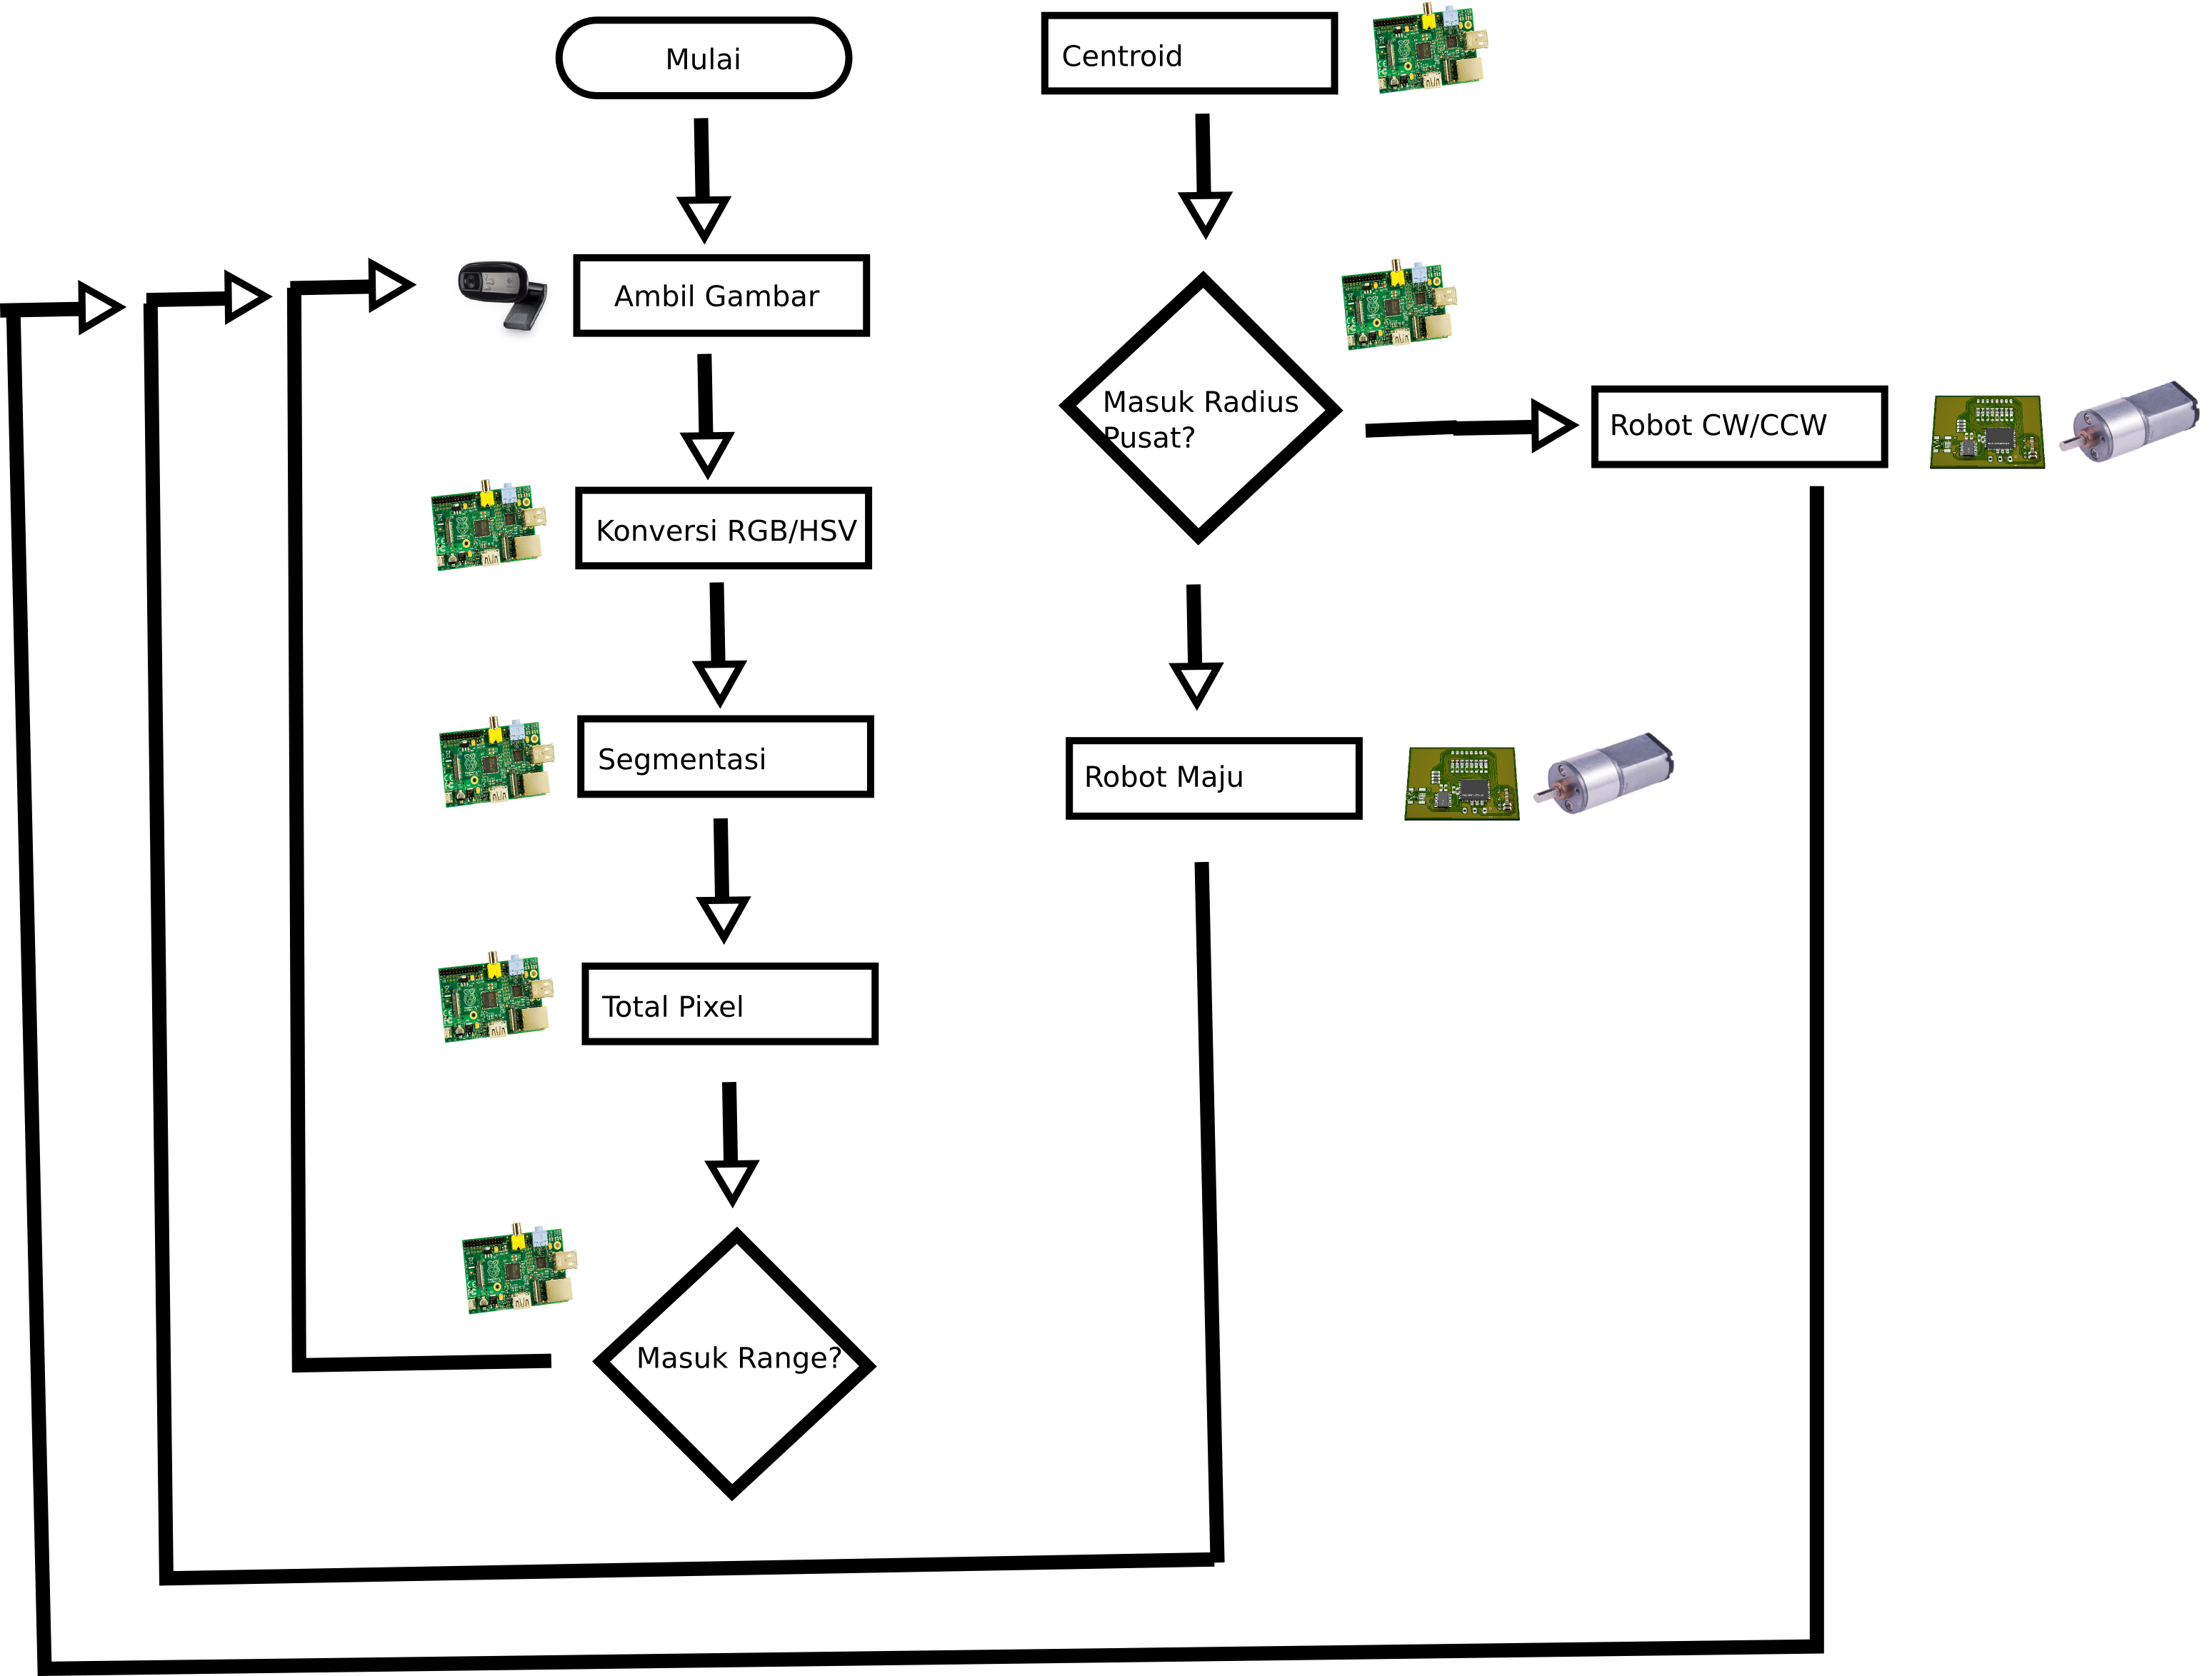
\includegraphics[width=250pt]{process}\\
    Gambar 1.4 rancangan algoritma perangkat lunak
  \end{center}
  
  Flowchart di atas beserta proses pengolahan citra telah dibentuk menjadi program/software yang dapat dijalankan di CPU.
  Program ini ditulis dengan C/C++ dan mampu membaca web camera untuk diolah berdasarkan nilai HSV yang telah ditentukan serta mampu memberi perintah ke Motor Controller.
  Gambar 1.5 berikut adalah tampilan perangkat lunak yang berjalan di RaspberrPi. 
  Perangkat lunak ini bekerja dengan mengambil dari kamera untuk kemudian diproses dan memutuskan aksi dari robot.
  
  \begin{center}
    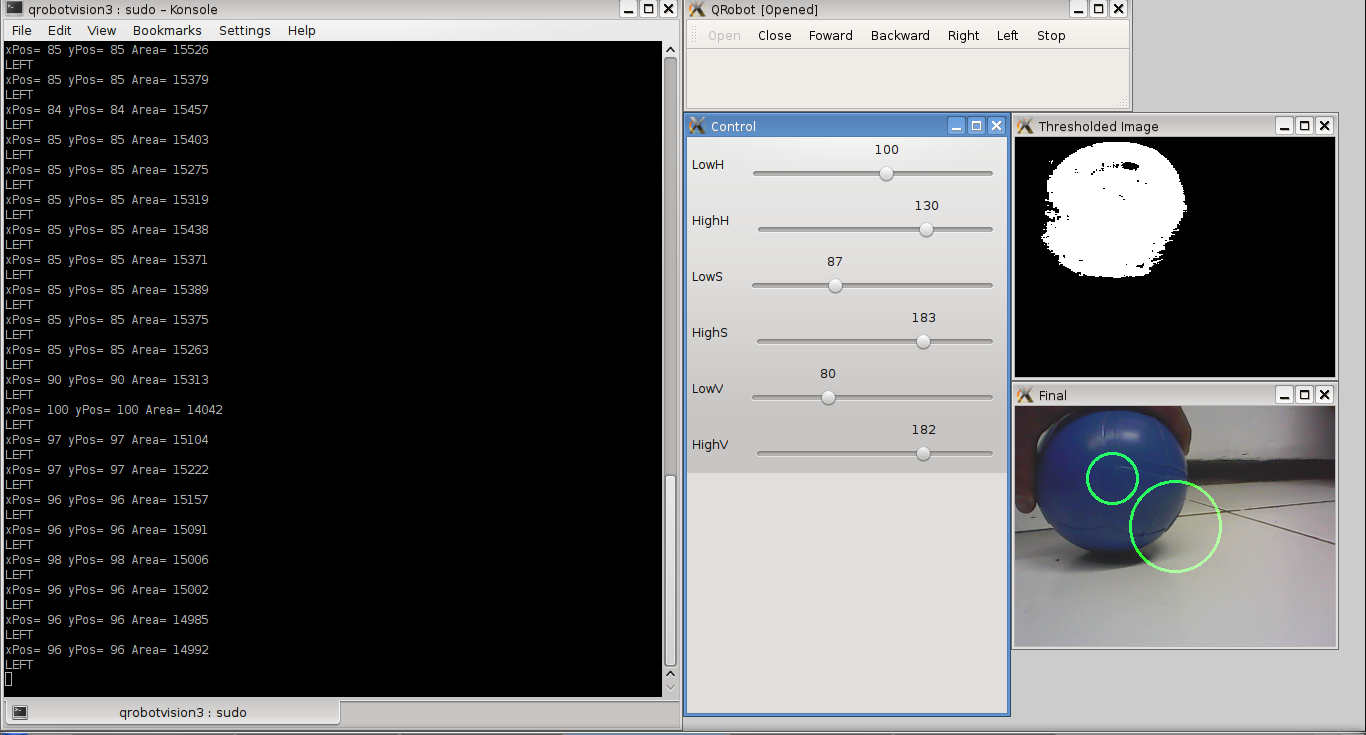
\includegraphics[width=250pt]{softpic}\\
    Gambar 2.5 Perangkat Lunak Robot
  \end{center}
  
  \begin{center}
     III. HASIL dan PEMBAHASAN
  \end{center}
  
  \noindent \textit{A. Field Of View (FOV)}
  
  Field Of View adalah batas jangkauan kiri dan kanan dari kamera yang dapat ditangkap gambarnya.
  Dalam lembar data dari web camera tertera bahwa FOV yang dimiliki adalah 58 derajat.
  Gambar 3.1 berikut menunjukkan skema posisi bola yang tertangkap kamera untuk menunjukkan nilai sudut FOV.
  \begin{center}
    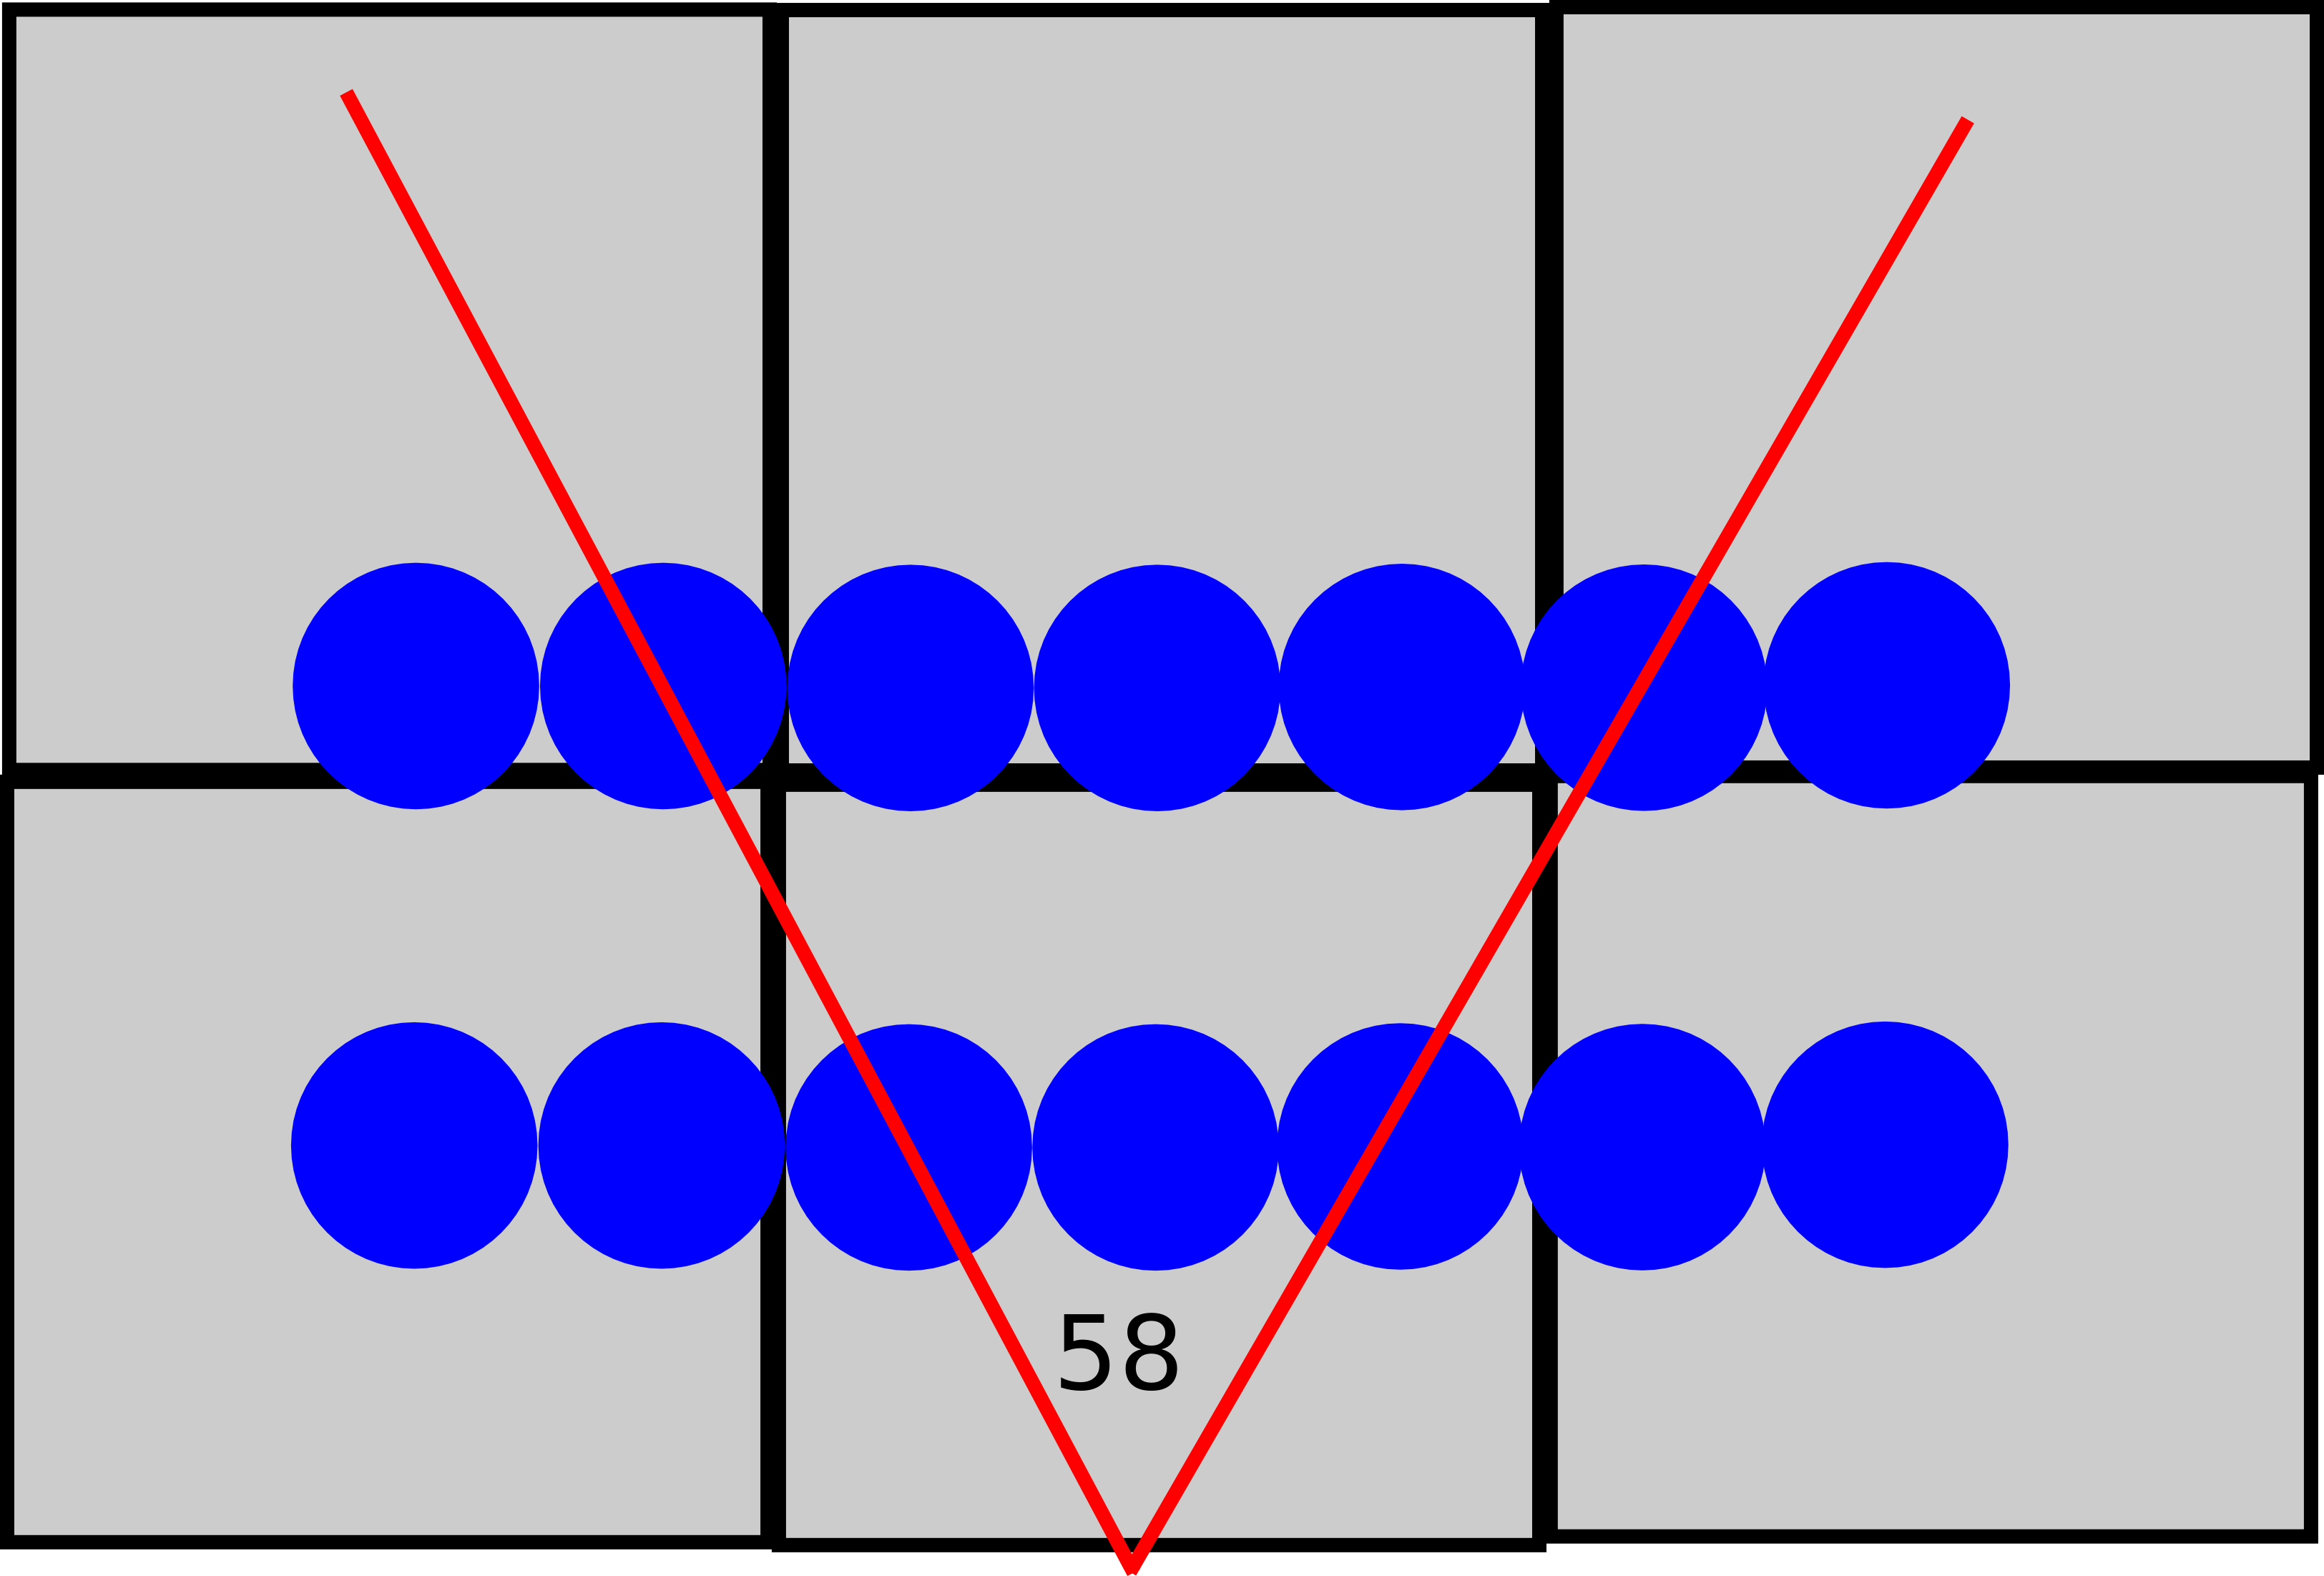
\includegraphics[width=200pt]{fov}\\
    Gambar 3.1 Skema FOV
  \end{center}
  Sedangkan gambar 3.2 berikut posisi bola yang tertangkap kamera
  \begin{center}
    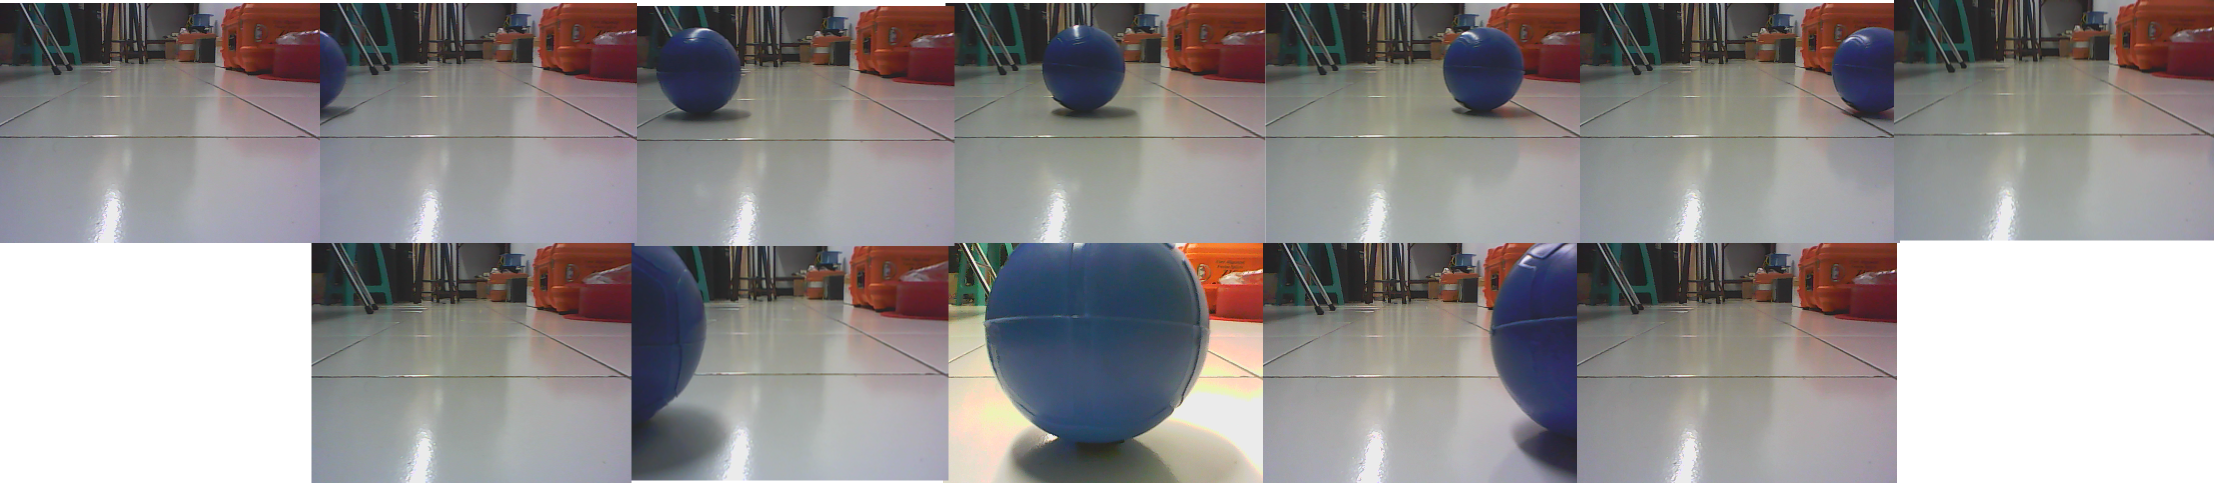
\includegraphics[width=200pt]{data_fov}\\
    Gambar 3.2 FOV
  \end{center}
  
  \noindent \textit{B. Range HSV}
  
  Untuk nilai range pada matrix Hue, telah ditetapkan nilainya oleh pustaka OpenCV.
  Untuk warna biru adalah antara 100-130.
  Sedangkan untuk nilai S dan V didapatkan dengan mengolah gambar mulai dari 0cm hingga 645 cm dengan kenaikan setiap 15cm diambil 10 gambar maka didapat 440 gambar.
  Setiap gambar diolah agar objek memiliki:\\
  - Jumlah pixel hasil threshold sebanyak mungkin\\
  - Posisi centroid yang masih di radius pusat gambar\\
 Pengolahan tersebut untuk mendapatkan jangkauan HSV sesuai kriteria di atas.
 
  Dengan mengambil rata-rata didapat bahwa nilai Smin adalah 87, Smax adalah 183, Vmin adalah 80, dan Vmax adalah 182.
  Nilai S dan V diatas kemudian digunakan dalam proses threshold.
  Apabila menggunakan nilai S dan V diatas, objek pada jarak lebih 585 cm sudah tidak lagi dapat dapat dibedakan antara pixel objek maupun pixel noise karena ukuran pixel objek relatif kecil.
  Kemudian nilai batas bawah dan atas jumlah pixel yang diambil adalah 31 dan 22500.
  
  \noindent \textit{C. Kecepatan}
  
  Pengujian kecepatan dilakukan untuk mendapatkan rentang kecepatan yang dapat diatur pada robot. 
  Motor robot secara default akan berputar dengan torsi 510 rpm dan torsi 15 kg.cm pada daya 12volt 1A. 
  Memberi daya kepada motor dalam pulsa dengan duty-cycle tertentu dapat mereduksi kecepatan motor agar sesuai dengan kebutuhan. 
  Tabel 3.1 adalah tabel hasil pengukuran rpm motor secara aktual dengan stroboscope pada setiap pengaturan duty-cycle.
  
  \begin{center}
   \begin{tabular}{ |l|l| }
    \hline
    Duty-Cycle & RPM\\
   \hline
    10 & 60\\
    20 & 126\\
    30 & 147\\
    40 & 200\\
    50 & 341\\
    60 & 398\\
    70 & 398\\
    80 & 397\\
    90 & 445\\
    100 & 510\\
    \hline
   \end{tabular}
   
  Tabel 3.1 Hasil pengujian duty-cycle
  \end{center}
  
  Selain mengalami reduksi rpm, motor dc juga mengalami reduksi torsi. 
  Berdasarkan pengujian dinamis diketahui bahwa pada duty-cycle 100\% robot gagal menemukan objek akibat gerakan yang terlalu cepat.
  Sedangkan pada 10\% robot tidak lagi bergerak
  Maka duty-cycle yang dapat digunakan adalah 20\% hingga 90\%.
  
  \noindent \textit{D. Pencahayaan}
  
  Pengujian ini ditujukan untuk menguji spesifikasi robot untuk melihat pengaruh tingkat pencahayaan pada pembacaan bola.
  Tingkat pencahayaan yang di ukur pada lumen 198, 74, 32, 17, 05 dan 0 (Gelap). 
  Setiap tingkat cahaya di ambil 10 foto sehingga total didapat 60 foto.
  Tabel 3.2 berikut menyajikan data rata-rata area pixel hasil threshold untuk setiap lumen.
  
    \begin{center}
   \begin{tabular}{ |l|l| }
    \hline
    Lumen & Pixel\\
   \hline
    198 & 1900\\
    74 & 14876\\
    32 & 15307\\
    17 & 15460\\
    05 & 9361\\
    0 & 0\\
    \hline
   \end{tabular}
  
  Tabel 3.2 Rata-rata jumlah pixel hasil threshold untuk setiap tingkat lumen.
 
  \end{center}
  
    Kemudian dengan bantuan perangkat lunak, setiap gambar diuji untuk melihat nilai HSV yang dimiliki pixel yang sama pada lumen yang berbeda
  Tabel 3.3 berikut menyajikan data HSV pada pixel yang sama namun pada lumen yang berbeda
  
   \begin{center}
   \begin{tabular}{ |l|l|l|l| }
    \hline
    Lumen & H & S & V\\
   \hline
    198 & 112  & 156  & 88 \\
    74  & 112  & 139  & 79 \\
    32  & 112  & 161  & 90 \\
    17  & 112  & 157  & 94 \\
    05  & 112  & 115  & 73 \\
    0   & 112  & 0    & 30 \\
    \hline
   \end{tabular}
   \end{center}
   
   Berdasarkan data di atas diketahui bahwa nilai Hue cenderung tetap yaitu pada nilai 112 kecuali pada lumen 0.
   Sedangkan yang mengalami perubahan adalah nilai saturasi dan value. 
   Seperti diketahui bahwa saturasi adalah tingkat suatu warna terhadap warna putih sehingga semakin gelapnya warna akan menurunkan tingkat saturasi, sedangkan value tingkat suatu warna terhadap warna hitam sehingga semakin cerahpnya warna akan menurunkan tingkat value\\

  \noindent \textit{E. Pemilihan Warna}
  
  Pengujian ini ditujukan untuk menguji spesifikasi robot dalam memilih warna. 
  Dalam pengujian ini, bola biru yang telah digunakan dalam pengujian-pengujian sebelumnya diletakkan berdekatan dengan tambahan 3 bola lain dengan warna merah, kuning dan hijau. 
  Gambar 3.3 berikut adalah gambar semua bola tersebut. 
  Untuk menguji robot dalam memilih warna biru, ke-empat bola tersebut diletakkan dalam 10 variasi posisi. 
  Gambar 3.4 menunjukkan 10 variasi tersebut. Robot tidak mengalami kegagalan dalam menemukan bola biru di setiap variasi posisi bola.

  \begin{center}
    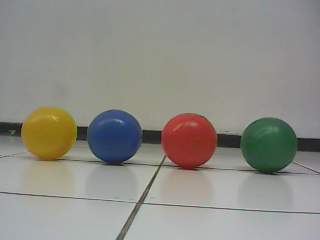
\includegraphics[width=200pt]{ball_all}\\
    Gambar 3.2 FOV
  \end{center}
  
  \begin{center}
    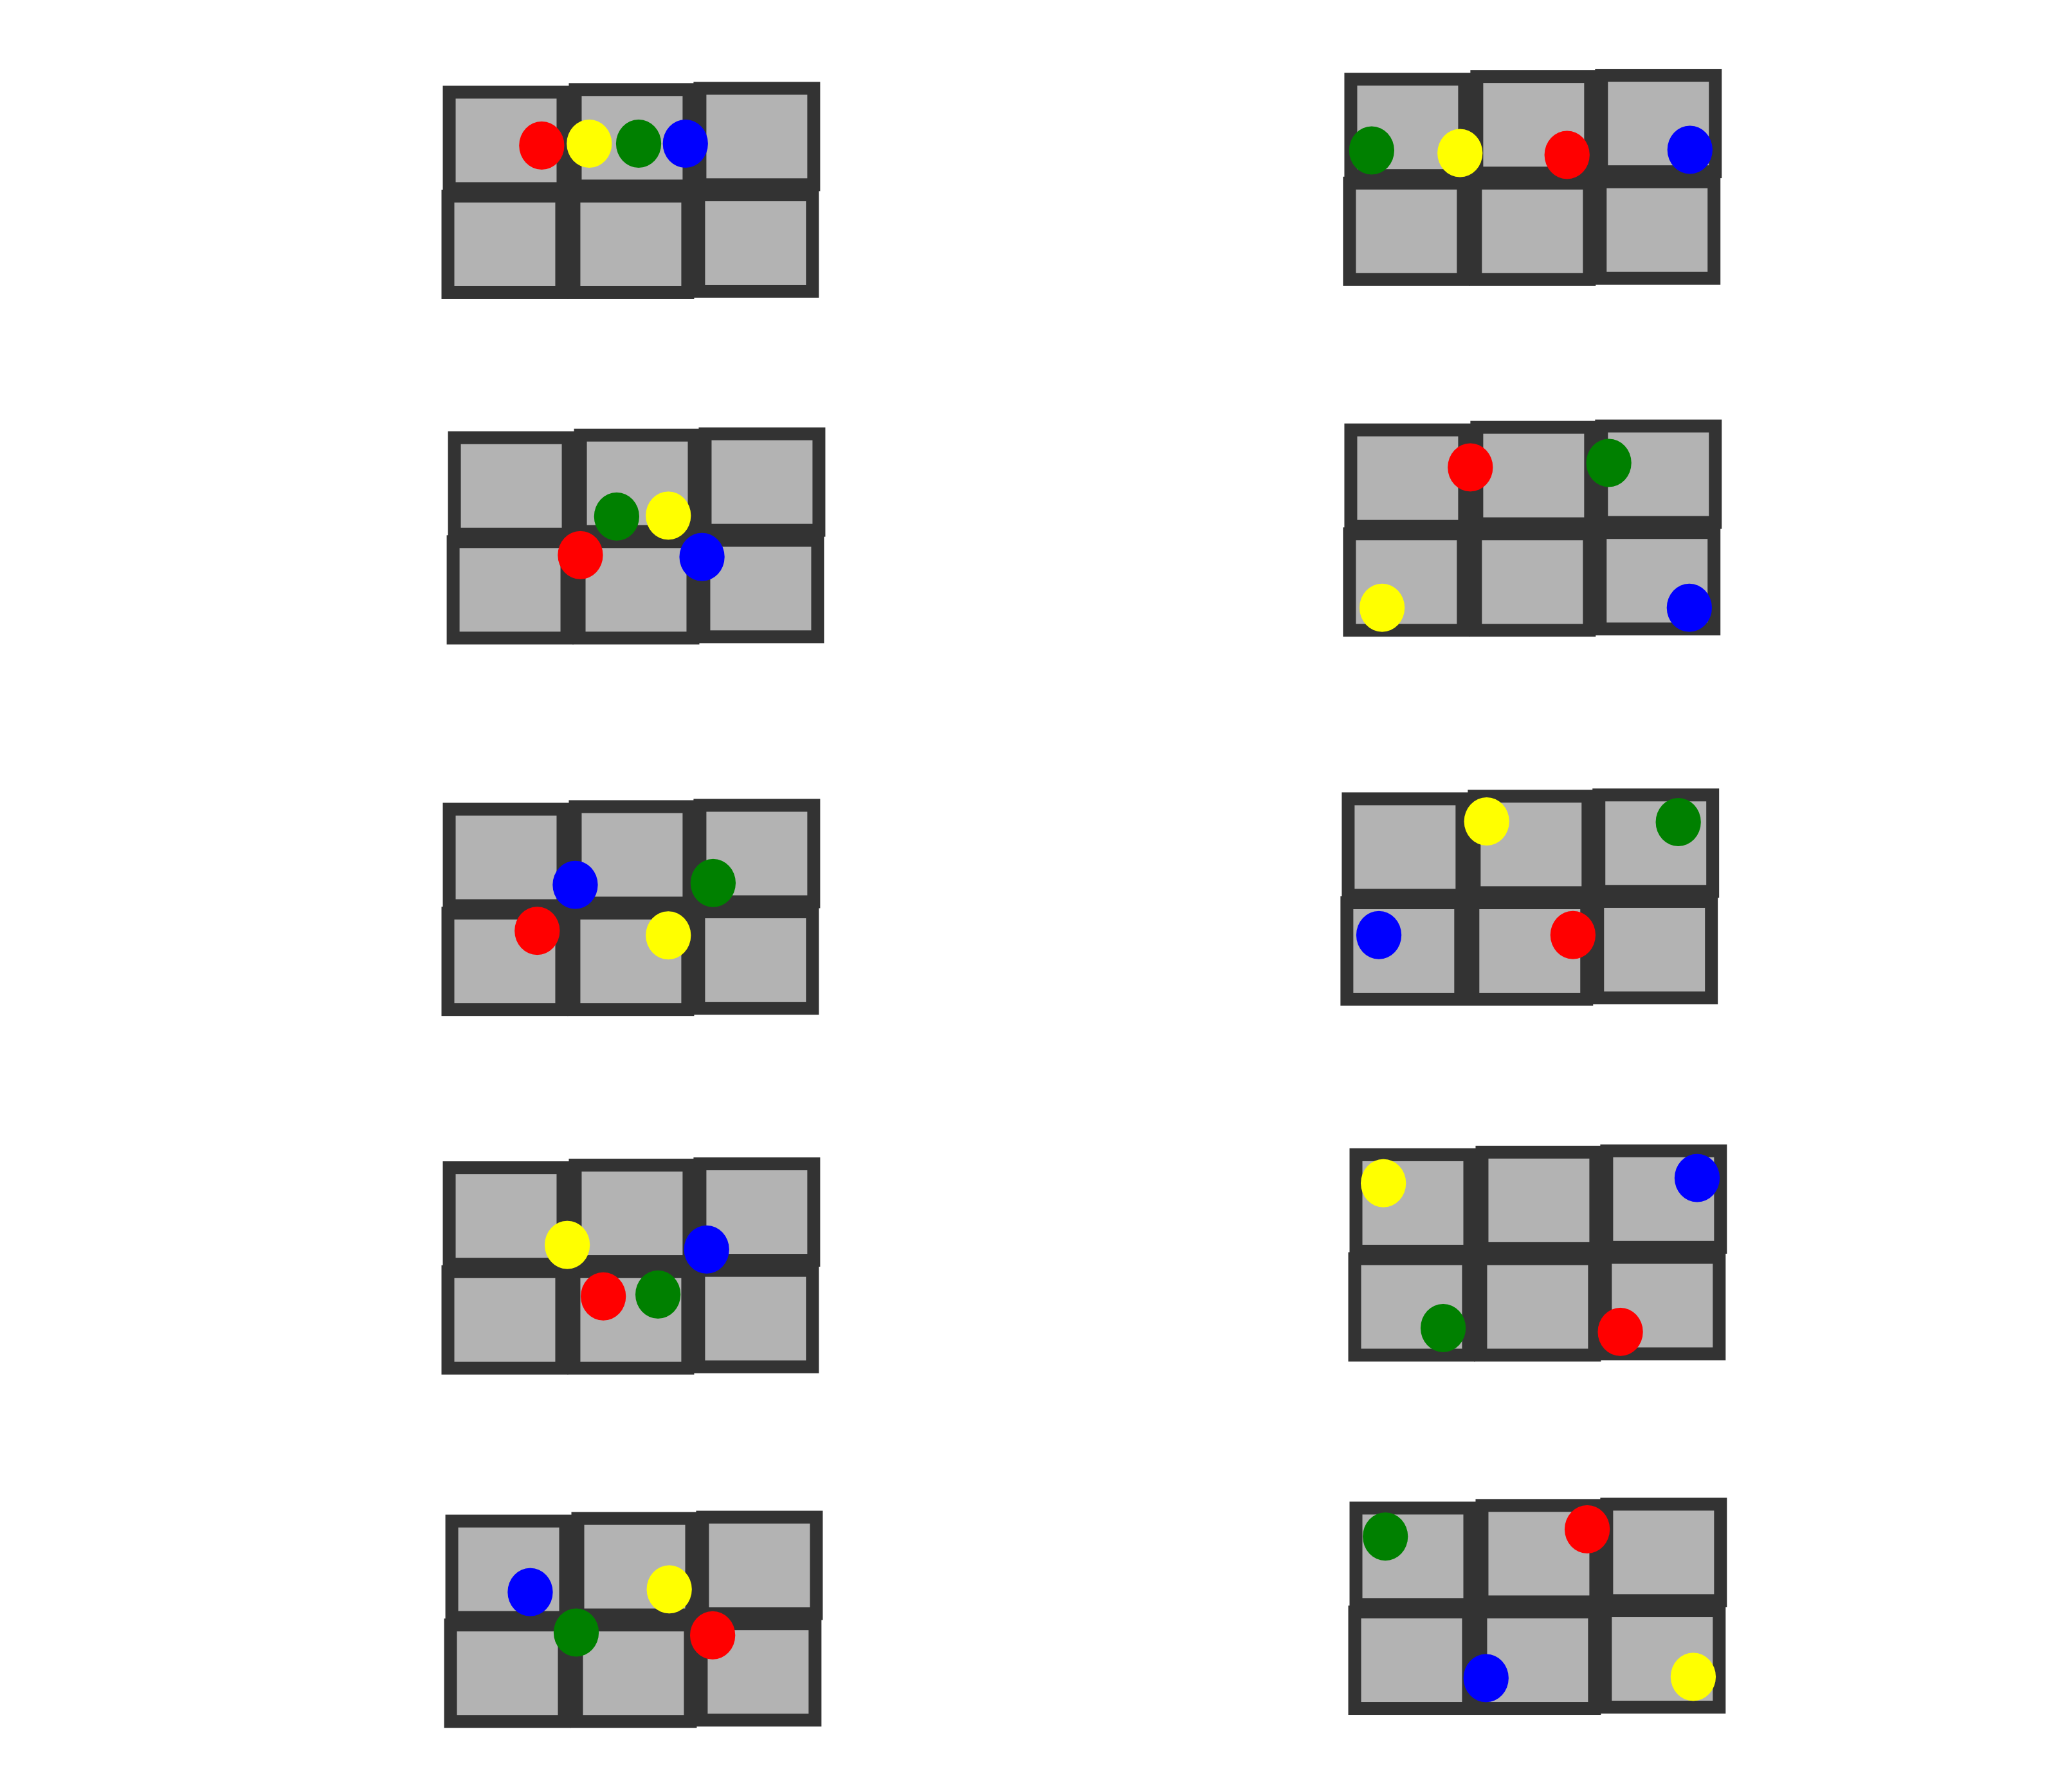
\includegraphics[width=200pt]{ball_pos}\\
    Gambar 3.4 Posisi bola
  \end{center}
  
  Kemudian dengan bantuan perangkat lunak dapat dilihat nilai HSV untuk setiap warna.
  Gambar 3.5 adalah perangkat lunak yang digunakan untuk melihat nilai HSV pada setiap bola
  Keempat bola memiliki rentang S dan V yang sama namun memiliki rentang H yang berbeda.
  Berdasarkan analisa di atas diketahui rentang Hue setiap bola adalah sebagai berikut:\\
  - Biru pada 100-130 \\
  - Hijau pada 60-90 \\
  - Kuning pada 15-35 \\
  - Merah pada 0-10 \\

  \begin{center}
    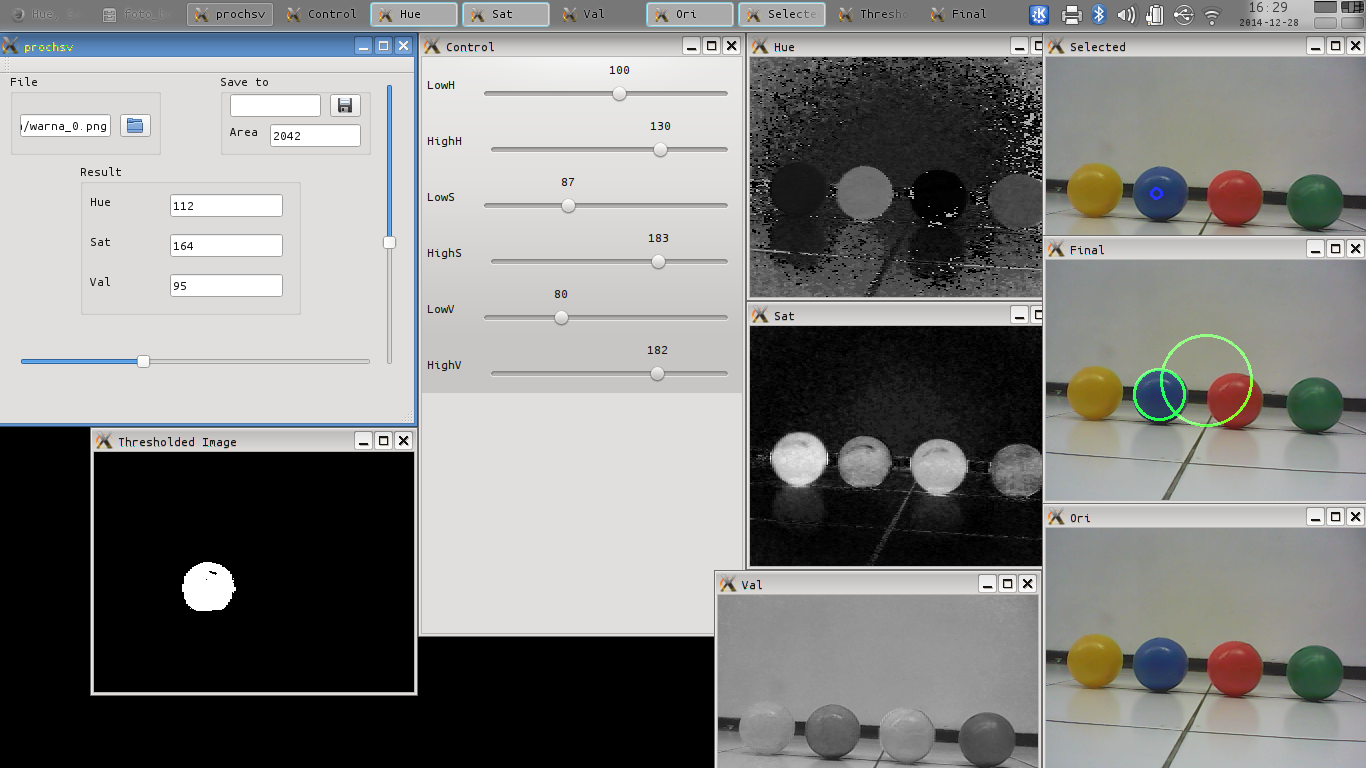
\includegraphics[width=200pt]{ball_color}\\
    Gambar 3.5 Mendapatkan nilai Hue
  \end{center}
  
  \begin{center}
     IV. PENUTUP
  \end{center}
  
  Dalam tugas akhir ini telah dirancang dan dibangun sebuah robot berbasis vision yang mampu menemukan objek. 
  Robot dapat menemukan objek dengan target adalah bola berwarna biru dengan pengaturan rentang Hue adalah 100-130, Saturation 87-183, dan Value 80-182.
  Dalam rentang ini robot dapat menemukan objek maximal pada jarak maximal 665 cm dan FOV 58 derajat dengan kecepatan roda antara 126-445 rpm. 
  Tingkat pencahayaan akan mempengaruhi nilai saturasi dan value. Untuk warna lain membedakannya cukup dengan nilai Hue yaitu untuk merah pada 0-10, kuning pada 15-35, dan hijau pada 60-90.
  
  \newpage
  
  \begin{center}
     V. DAFTAR PUSTAKA
  \end{center}
  
  - Aleš Ude " \textit{Robot Vision} " 2010\\
  - Andor Team " \textit{Digital Camera Fundamentals} " 2012\\
  - Browning, Brett " \textit{Real-Time, Adaptive Color-based Robot Vision} " 2013\\
  - Chao, Fei " \textit{A developmental approach to robotic pointing via human–robot interaction} " 2014\\
  - Honda Team " \textit{Asimo Technical Information} " 2007\\
  - Aldebaran Robotics " \textit{Nao Technical Datasheet} " 2012\\
  - Robotis " \textit{Darwin-Op Technical Manual} " 2012\\
  - Upton, Eben " \textit{RaspberryPi User Guide} " 2012\\
  - OpenCV Team " \textit{The OpenCV Reference Manual} " 2014\\
  - Phillips, Dwyne " \textit{Image Processing in C} " 2000\\
  - Zhou, Huiyu " \textit{Digital Image Processing Part I} " 2010\\

\end{document}
